\chapter{Background}                                \label{Chapter:background}


% ===================================================================================================
% === NEW SECTION === NEW SECTION === NEW SECTION === NEW SECTION === NEW SECTION === NEW SECTION ===
% ===================================================================================================
\section{Transdermal drug delivery}                 \label{Chapter:background/transdermal drug delivery}
    % \subsection{Problems}                           \label{Chapter:background/transdermal drug delivery/problems}
    % \subsection{Alternative methods}                \label{Chapter:background/transdermal drug delivery/alternative methods}

    Transdermal drug delivery is a method of delivery for pharmaceutical solutions that are unsuitable for ingestion or cannot penetrate through the skin. Many vaccines and insulin are delivered by this approach\,\cite{sadrzadeh2007}. While being efficient and precise, transdermal drug delivery via hypodermic needle is time-consuming, labor intensive, and hazardous. The procedure requires the operator to attach a hollow needle to a syringe, then extract the drug, eliminate air bubbles in the syringe and sterilize the applied area thoroughly. Once prepared, the operator can slowly inject a high volume of drug. During disposal, needle stick is a safety hazard. Needle-stick injuries hold a high risk of transmitting contagious diseases such as HIV, HBV, and HCV. Percutaneous sharps injuries affected millions of individuals across the world\,\cite{pruss2005}. 
    
    Today, needle sticks and sharp objects still represent a significant challenge in creating a safe environment for professional health care practitioners. Pain\,\cite{schneider1994} and needle-phobia\,\cite{hamilton2005,Nir2003} are other motivations to develop and popularize alternative strategies.
    
    Some distinct transdermal drug delivery methods were invented to tackle issues of needle injection. They include iontophoresis\,\cite{dhote2012}, sonophoresi\,\cite{bommanan1992}, permeation enhancement by chemicals\,\cite{karande2006}, micro-needles on patch\,\cite{cormier2004}, and jet injection\,\cite{taberner2006}. 

% ===================================================================================================
% === NEW SECTION === NEW SECTION === NEW SECTION === NEW SECTION === NEW SECTION === NEW SECTION ===
% ===================================================================================================
\section{Needle-free Jet Injection}                 \label{Chapter:background/needle-free jet injection}
    
    
    % -----------------------------------------------------------------------------------
    % --- NEW SUB SECTION --- NEW SUB SECTION --- NEW SUB SECTION --- NEW SUB SECTION --- 
    % -----------------------------------------------------------------------------------
    \subsection{How it works}                       \label{Chapter:background/needle-free jet injection/how it works}
    
        \ac{NFJI}, commonly called “hypo-spray” in science fiction, was patented in 1960\,\cite{ismach1962}. Figure\,\ref{fig:chapter/background/explain needle free/original injector} shows the original \acs{NFJI} device, “Ped-O-Jet” in use for the purpose of mass vaccination\,\cite{DictionnairesetEncyclopediessurAcademic}. This device was invented  upon realizing that pressurized fluid can penetrate human skins. Fluid streams of appropriate diameter and velocity can produce sufficient pressure to breach through the skin layers up to a particular desired depth. 
        
        \begin{figure*}[!ht]
            \centering
            \subfloat[Ped-O-Jet in use.]{
                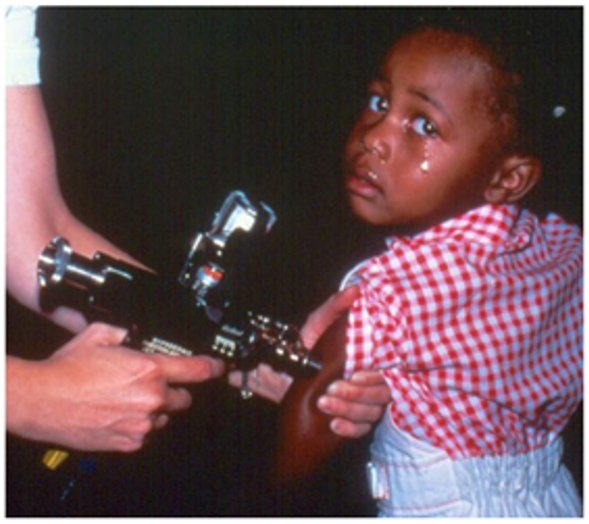
\includegraphics[width=0.35\textwidth]{chap2/images/original_injector.png}
                \label{fig:chapter/background/explain needle free/original injector}
            }
            \qquad
            \subfloat[Needle injection versus Needle-free injection]{
                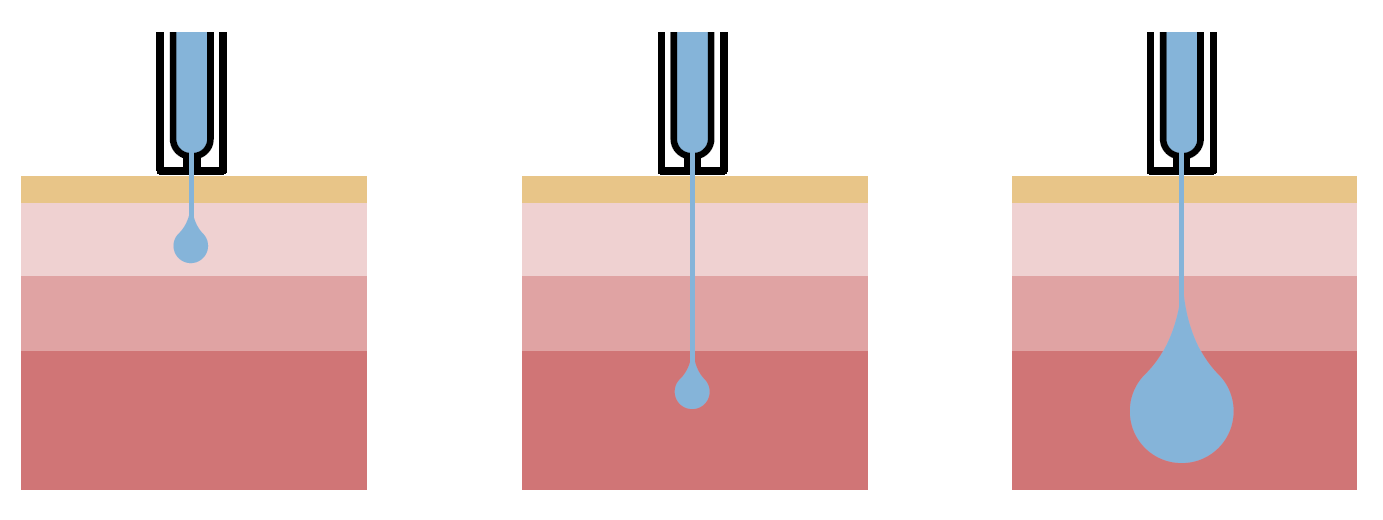
\includegraphics[width=0.45\textwidth]{chap2/images/needle_vs_needle_free.png}
                \label{fig:chapter/background/explain needle free/needle vs no needle}
            }
            \caption{
                Two different style of optimization objective function evaluation.
            }   \label{fig:chapter/background/explain needle free}
        \end{figure*}
        
        A subcutaneous or intramuscular jet injection could be realized by forcing a fluid jet of $\mathrm{76-360\,\mu m}$  diameter to penetrate the human skin at a speed faster than $\mathrm{100 m/s}$\,\cite{mitragotri2006,Hogan2006}. Figure\,\ref{fig:chapter/background/explain needle free/needle vs no needle} shows that an ideal jet injection would deliver the drug in a similar manner to which of a hypodermic needle injection\,\cite{InsuJet2013}.
        
        % Even though this method adopts the use of needle-free apparatus, biological material can still be unwillingly transferred if there are no appropriate decontamination schemes. Concerns have been raised in the literature about potential transmission of blood-borne infections by multiple-use \acs{NFJI} since the early 1970s\,\cite{kremer1970, weintraub1988}. Figure\,\ref{fig:chapter/background/injection mechanism} illustrates three possible mechanisms of how blood contamination can take place\,\cite{hoffman2001}. 
        
        % \begin{figure*}[!ht]
    
        %     \centering
        %     \subfloat[]{
        %         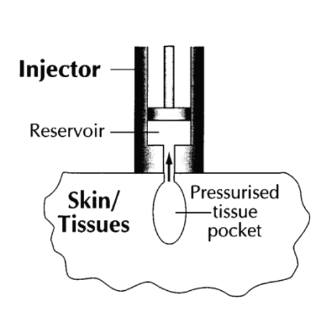
\includegraphics[width=0.29\textwidth]{chap2/images/jet_injection_mechanism_1.png}
        %         \label{fig:chapter/background/injection mechanism/1}
        %     }
        %     \subfloat[]{
        %         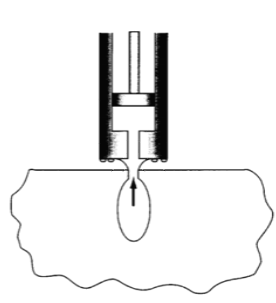
\includegraphics[width=0.25\textwidth]{chap2/images/jet_injection_mechanism_2.png}
        %         \label{fig:chapter/background/injection mechanism/2}
        %     }
        %     \subfloat[]{
        %         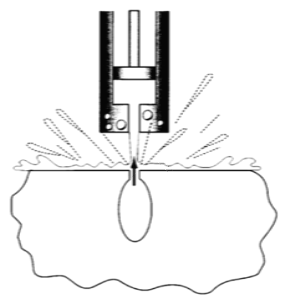
\includegraphics[width=0.27\textwidth]{chap2/images/jet_injection_mechanism_3.png}
        %         \label{fig:chapter/background/injection mechanism/3}
        %     }
        %     \caption{
        %         3 possible mechanisms of blood contamination in ‘mass campaign jet injectors’. 
        %     }   \label{fig:chapter/background/injection mechanism}
        % \end{figure*}    
        
        % Scenario in Figure\,\ref{fig:chapter/background/injection mechanism/1} shows that tissues return fluid into the reservoir as injection pressure diminishes. Liquid flows out to the tip of the injector as the injector’s tip is removed from the applied area as illustrated in Figure\,\ref{fig:chapter/background/injection mechanism/2}. Scenario in Figure\,\ref{fig:chapter/background/injection mechanism/3} displays a ‘splash back’ of jet stream during injection. Uninterrupted, continuous, reuse of \acs{NFJI} has historically caused instances of mass HBV spread\,\cite{canter1990}. For prevention of future mass infection, ‘mass campaign jet injectors’ were disapproved for human use by the World Health Organization\,\cite{who2005}. Nowadays, reusable \acsp{NFJI} for human use must accommodate replaceable syringes. 
    
    
    % -----------------------------------------------------------------------------------
    % --- NEW SUB SECTION --- NEW SUB SECTION --- NEW SUB SECTION --- NEW SUB SECTION --- 
    % -----------------------------------------------------------------------------------
    \subsection{Commercially available options}     \label{Chapter:background/needle-free jet injection/commercially available options}
        
        Commercially available \acsp{NFJI} including BIOJECT Zeajet\footnote{http://www.bioject.com/products/zetajet-info} , INJEX 30\footnote{https://www.injex.com.au/injex/injex} , PHARMAJET Stratis\footnote{http://pharmajet.com/fda-approved-needleless-flu-shot} , COMFORT-IN\footnote{http://www.comfort-in.com/diabetes.html}  are spring-powered, small, portable, and handheld devices. They are capable of delivering either vaccination or insulin in a small dose, with volume limited to $\mathrm{300\,\mu L}$. Figure 3 illustrates the appearance, construction, and mechanism of the spring-loaded PHARMAJET Stratis NFJI as an example. These devices come in various shapes, sizes, injection volumes, and target skin layers. However, their primary structure consists of three main components:
        \begin{itemize}
            \item Energy storage - compressed gas, spring coil or explosives\,\cite{taberner2012}, which are often accompanied by a recharging device,
            \item Piston - actuator with various size and triggering method to accomplish desired pressure profile as well as injection volume specification,
            \item Replaceable syringe - single use container with orifice hole diameter of under $\mathrm{1\,mm}$.
        \end{itemize}
        
        Once triggered, stored energy produces varying pressure on the injection cylinder until the piston reaches the end of its track. Different devices utilize different recoil or trigger mechanisms, but no system is capable of monitoring and measuring injection performance. Instead of concentrated fluid delivery in a narrow stream down the tissue, these devices tend to spread the drug content in a cone shape\,\cite{baxtex2005}. Figure\,\ref{fig:chapter/background/jet injection effectiveness/mechanical devices pressure curve} shows the sharp peak and oscillating nature of the pressure produced by injection stream of a BIOJECT Vitajet 3™ spring powered \acsp{NFJI}\,\cite{schramm2002}. Schneider et. al.\,\cite{schneider1994} reported that without stroke velocity and position control, the sharp fluid pressure profile peak could cause pain, bruises, bleeding, and blisters. Their studies also showed evidence that the same spring powered NFJI device exhibits inconsistent performance across different skin types and conditions. 
        
        Despite being a safer alternative, mechanically powered \acsp{NFJI} require manual recharging. Thus, the average cycle time was recorded to be no faster than that of a conventional hypodermic needle injection\,\cite{PharmaJet2011}. More advanced \acsp{NFJI} like LECTRAJET  have shown the capability of automatic spring recoil to reduce reload time. Lack of pressure control, low injection volume (typically $0.05$ to $0.3\,\mathrm{mL}$), long cycle time, poor repeatability and reproducibility are drawbacks of commercially available mechanically powered \acsp{NFJI}.
        
        \begin{figure*}[!ht]
            \centering
            \subfloat[Typical pressure curve for a $152\,\mathrm{\mu m}$ diameter nozzle from injector Vitajet\,3™]{
                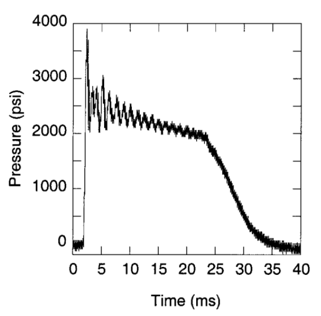
\includegraphics[width=0.43\textwidth]{chap2/images/jet_injection_pressure_curve.png}
                \label{fig:chapter/background/jet injection effectiveness/mechanical devices pressure curve}
            }
            \qquad
            \subfloat[Delivery of mannitol by jet injection into human (A), porcine abdominal (B), and porcine dorsal skin (C) using the same device at $177\,\mathrm{m/s}$. There is a significant difference between each type of skin tested ($p=0.001$)]{
                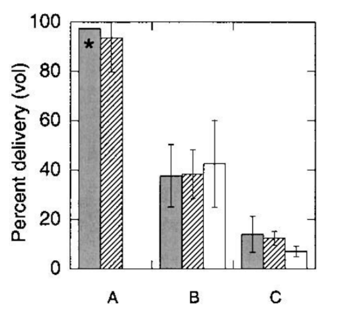
\includegraphics[width=0.45\textwidth]{chap2/images/jet_injection_delivery_study.png}
                \label{fig:chapter/background/jet injection effectiveness/delivery statistic}
            }
            \caption{
                Results of different jet injection study on mechanically powered \acs{NFJI} devices.
            }   \label{fig:chapter/background/jet injection effectiveness/}
        \end{figure*}


    % -----------------------------------------------------------------------------------
    % --- NEW SUB SECTION --- NEW SUB SECTION --- NEW SUB SECTION --- NEW SUB SECTION --- 
    % -----------------------------------------------------------------------------------
    \subsection{Controllable \acs{NFJI} devices}    \label{Chapter:background/needle-free jet injection/Controllable NFJI}
    
        Recent achievements in high power density actuators enabled successful prototypes of electronic controlled \acsp{NFJI} which were capable of real-time jet velocity control. Hemond et. al. [24] suggests four advantages of electronics control over traditional needle injection and mechanically powered jet injection:
        
        \begin{itemize}
            \item Controllable - capable of maintaining high pressure without the need of trading-off for injection volume,
            \item Reliable - capable of producing consistent jet pressure on a broad range of skin properties and different injection types,
            \item Versatile - automatic reload under closed loop control or injection volume control,
            \item Measurable - convenient in monitoring progress to evaluate the performance of injection.
        \end{itemize}
        
        This class of device performs injections by utilizing different electrically powered actuators: dynamically controlled piezo-electric actuators\,\cite{Stachowiak2009}, laser pulsed microjets\,\cite{tawaga2013, park2012} and Lorentz force voice coil motors\,\cite{taberner2006,hemond2006}. Piezo-electric and laser pulse methods are limited to sub $\mathrm{\mu L}$ injections. Scaling of Piezo-electric technology to   range in injection volume appear ambitious. Cumbersome ‘off-the-shelf’ voice coil actuators are not yet suitable to become handheld.

% ===================================================================================================
% === NEW SECTION === NEW SECTION === NEW SECTION === NEW SECTION === NEW SECTION === NEW SECTION ===
% ===================================================================================================
\section{Voice coil motors for NFJI}                \label{Chapter:background/voice coil motors for NFJI}
    \subsection{How it works}                       \label{Chapter:background/voice coil motors for NFJI/how it works}
    \subsection{Past work}                          \label{Chapter:background/voice coil motors for NFJI/past work}
    \subsection{Scaling properties}                 \label{Chapter:background/voice coil motors for NFJI/scaling properties}
    \subsection{Limitations}                        \label{Chapter:background/voice coil motors for NFJI/Limitations}


% ===================================================================================================
% === NEW SECTION === NEW SECTION === NEW SECTION === NEW SECTION === NEW SECTION === NEW SECTION ===
% ===================================================================================================
\section{Linear synchronous motors for NFJI}        \label{Chapter:background/linear synchronous motors for NFJI}
    \subsection{Classification}                     \label{Chapter:background/linear synchronous motors for NFJI/classification}
    \subsection{Advantages}                         \label{Chapter:background/linear synchronous motors for NFJI/advantages}
    \subsection{Challenges}                         \label{Chapter:background/linear synchronous motors for NFJI/challenges}


% ===================================================================================================
% === NEW SECTION === NEW SECTION === NEW SECTION === NEW SECTION === NEW SECTION === NEW SECTION ===
% ===================================================================================================
\section{Electromagnetic field theory}              \label{Chapter:background/electromagnetic field theory}
    \subsection{Quasi-static Maxwell equations}     \label{Chapter:background/electromagnetic field theory/quasi-static maxwell equations}
    \subsection{Ferromagnetic materials}            \label{Chapter:background/electromagnetic field theory/ferromagnetic materials}
    \subsection{Materials for motor construction}   \label{Chapter:background/electromagnetic field theory/materials for motor construction}


% ===================================================================================================
% === NEW SECTION === NEW SECTION === NEW SECTION === NEW SECTION === NEW SECTION === NEW SECTION ===
% ===================================================================================================
\section{Modelling techniques for motors}           \label{Chapter:background/modelling techniques for designing motors}
    \subsection{Numerical methods}                  \label{Chapter:background/modelling techniques for designing motors/numerical methods}
    \subsection{Analytical methods}                 \label{Chapter:background/modelling techniques for designing motors/analytical methods}
    \subsection{Semi-analytical methods}            \label{Chapter:background/modelling techniques for designing motors/semi-analytical methods}
    \subsection{Empirical methods}                  \label{Chapter:background/modelling techniques for designing motors/empirical methods}


% ===================================================================================================
% === NEW SECTION === NEW SECTION === NEW SECTION === NEW SECTION === NEW SECTION === NEW SECTION ===
% ===================================================================================================
\section{Optimization methods}                      \label{Chapter:background/optimization methods}
    \subsection{Classification}                     \label{Chapter:background/optimization methods/classification}
    \subsection{Application in motor design}        \label{Chapter:background/optimization methods/application in motor design}


% ===================================================================================================
% === NEW SECTION === NEW SECTION === NEW SECTION === NEW SECTION === NEW SECTION === NEW SECTION ===
% ===================================================================================================
\section{Summary}                                   \label{Chapter:background/summary}